% 注意事项:编译两次,以确保目录、页码完整显示

\def\allfiles{}

\documentclass[14pt,a4paper,UTF8,twoside]{article}

% Formatting Packages ——————————————————————————————————————
\usepackage{multicol}
\usepackage{multirow}
\usepackage{enumitem}
\usepackage{indentfirst}
\usepackage[toc]{multitoc}

% Math & Physics Packages ————————————————————————————
\usepackage{amsmath, amsthm, amsfonts, amssymb}
\usepackage{setspace}
\usepackage{physics}
\usepackage{cancel}
\usepackage{nicefrac}
\usepackage{unicode-math} % 允许数学公式使用特定字体

% Image-related Packages —————————————————————————————
\usepackage{float} % 浮动体环境
\usepackage{subcaption} % 子图包
\usepackage{graphics, graphicx}
\usepackage{tikz, tikz-qtree}
\usepackage{mdframed}
\usepackage{lmodern}
\usetikzlibrary{arrows.meta}
\usetikzlibrary{shapes.geometric, arrows}
\tikzstyle{node_style} = [rectangle, rounded corners, draw, align=center, text width=3cm, minimum height=0.65cm]
\tikzstyle{arrow_style} = [thick, ->, >=stealth]

\usepackage{pgfplots}
\pgfplotsset{compat=1.18}
\usepackage{xcolor}
\usepackage{fourier-orns}
\usepackage{lipsum}

% Colour Palette ——————————————————————————————————————
\definecolor{merah}{HTML}{F4564E}
\definecolor{merahtua}{HTML}{89313E}
\definecolor{biru}{HTML}{60BBE5}
\definecolor{birutua}{HTML}{412F66}
\definecolor{hijau}{HTML}{59CC78}
\definecolor{hijautua}{HTML}{366D5B}
\definecolor{kuning}{HTML}{FFD56B}
\definecolor{jingga}{HTML}{FBA15F}
\definecolor{ungu}{HTML}{8C5FBF}
\definecolor{lavender}{HTML}{CBA5E8}
\definecolor{merjamb}{HTML}{FFB6E0}
\definecolor{mygray}{HTML}{E6E6E6}
\definecolor{mygreen}{rgb}{0,0.6,0}
\definecolor{mymauve}{rgb}{0.58,0,0.82}

% Theorems ————————————————————————————————————————————
\usepackage{tcolorbox}
\usepackage{changepage}
\tcbuselibrary{skins,breakable,theorems}

\newcounter{hitung}
\setcounter{hitung}{\thesection}

\makeatletter
	% Proof 证明如下
	\def\tcb@theo@widetitle#1#2#3{\hbox to \textwidth{\textsc{\large#1}\normalsize\space#3\hfil(#2)}}
	\tcbset{
		theorem style/theorem wide name and number/.code={ \let\tcb@theo@title=\tcb@theo@widetitle},
		proofbox/.style={skin=enhancedmiddle,breakable,parbox=false,boxrule=0mm,
			check odd page, toggle left and right, colframe=black!20!white!92!hijau,
			leftrule=8pt, rightrule=0mm, boxsep=0mm,arc=0mm, outer arc=0mm,
			left=3mm,right=3mm,top=0mm,bottom=0mm, toptitle=0mm,
			bottomtitle=0mm,colback=gray!3!white!98!biru, before skip=8pt, after skip=8pt,
			before={\par\vskip-2pt},after={\par\smallbreak},
		},
	}
	\newtcolorbox{ProofBox}{proofbox}
	\makeatother
	
	\let\realproof\proof
	\let\realendproof\endproof
	\renewenvironment{proof}[1][Prove:]{\ProofBox\strut\textsc{#1}\space}{\endProofBox}
        \AtEndEnvironment{proof}{\null\hfill$\blacksquare$}
        % Definition 定义环境
	\newtcbtheorem[use counter=hitung, number within=section]{dfn}{定义}
	{theorem style=theorem wide name and number,breakable,enhanced,arc=3.5mm,outer arc=3.5mm,
		boxrule=0pt,toprule=1pt,leftrule=0pt,bottomrule=1pt, rightrule=0pt,left=0.2cm,right=0.2cm,
		titlerule=0.5em,toptitle=0.1cm,bottomtitle=-0.1cm,top=0.2cm,
		colframe=white!10!biru,
		colback=white!90!biru,
		coltitle=white,
		shadow={1.3mm}{-1.3mm}{0mm}{gray!50!white}, % 添加阴影
        coltext=birutua!60!gray, title style={white!10!biru}, rbefoe skip=8pt, after skip=8pt,
		fonttitle=\bfseries,fontupper=\normalsize}{dfn}

	% 答题卡
	\newtcbtheorem[use counter=hitung, number within=section]{ans}{解答}
	{theorem style=theorem wide name and number,breakable,enhanced,arc=3.5mm,outer arc=3.5mm,
		boxrule=0pt,toprule=1pt,leftrule=0pt,bottomrule=1pt, rightrule=0pt,left=0.2cm,right=0.2cm,
		titlerule=0.5em,toptitle=0.1cm,bottomtitle=-0.1cm,top=0.2cm,
		colframe=white!10!biru,
		colback=white!90!biru,
		coltitle=white,
		shadow={1.3mm}{-1.3mm}{0mm}{gray!50!white}, % 添加阴影
        coltext=birutua!60!gray, title style={white!10!biru}, before skip=8pt, after skip=8pt,
		fonttitle=\bfseries,fontupper=\normalsize}{ans}

	% Axiom
	\newtcbtheorem[use counter=hitung, number within=section]{axm}{公理}
	{theorem style=theorem wide name and number,breakable,enhanced,arc=3.5mm,outer arc=3.5mm,
		boxrule=0pt,toprule=1pt,leftrule=0pt,bottomrule=1pt, rightrule=0pt,left=0.2cm,right=0.2cm,
		titlerule=0.5em,toptitle=0.1cm,bottomtitle=-0.1cm,top=0.2cm,
		colframe=white!10!biru,colback=white!90!biru,coltitle=white,
		shadow={1.3mm}{-1.3mm}{0mm}{gray!50!white!90}, % 添加阴影
        coltext=birutua!60!gray,title style={white!10!biru},before skip=8pt, after skip=8pt,
		fonttitle=\bfseries,fontupper=\normalsize}{axm}
 
	% Theorem
	\newtcbtheorem[use counter=hitung, number within=section]{thm}{定理}
	{theorem style=theorem wide name and number,breakable,enhanced,arc=3.5mm,outer arc=3.5mm,
		boxrule=0pt,toprule=1pt,leftrule=0pt,bottomrule=1pt, rightrule=0pt,left=0.2cm,right=0.2cm,
		titlerule=0.5em,toptitle=0.1cm,bottomtitle=-0.1cm,top=0.2cm,
		colframe=white!10!merah,colback=white!75!pink,coltitle=white, coltext=merahtua!80!merah,
		shadow={1.3mm}{-1.3mm}{0mm}{gray!50!white!90}, % 添加阴影
		title style={white!10!merah}, before skip=8pt, after skip=8pt,
		fonttitle=\bfseries,fontupper=\normalsize}{thm}
	
	% Proposition
	\newtcbtheorem[use counter=hitung, number within=section]{prp}{命题}
	{theorem style=theorem wide name and number,breakable,enhanced,arc=3.5mm,outer arc=3.5mm,
		boxrule=0pt,toprule=1pt,leftrule=0pt,bottomrule=1pt, rightrule=0pt,left=0.2cm,right=0.2cm,
		titlerule=0.5em,toptitle=0.1cm,bottomtitle=-0.1cm,top=0.2cm,
		colframe=white!10!hijau,colback=white!90!hijau,coltitle=white, coltext=hijautua!80!brown,
		shadow={1.3mm}{-1.3mm}{0mm}{gray!50!white}, % 添加阴影
		title style={white!10!hijau}, before skip=8pt, after skip=8pt,
		fonttitle=\bfseries,fontupper=\normalsize}{prp}


	% Example
	\newtcolorbox[use counter=hitung, number within=section]{cth}[1][]{breakable,
		colframe=white!10!jingga, coltitle=white!90!jingga, colback=white!85!jingga, coltext=black!10!brown!50!jingga, colbacktitle=white!10!jingga, enhanced, fonttitle=\bfseries,fontupper=\normalsize, attach boxed title to top left={yshift=-2mm}, before skip=8pt, after skip=8pt,
		title=Contoh~\thetcbcounter \ \ #1}

	% Catatan/Note
	\newtcolorbox{ctt}[1][]{enhanced, 
		left=4.1mm, borderline west={8pt}{0pt}{white!10!kuning}, 
		before skip=6pt, after skip=6pt, 
		colback=white!85!kuning, colframe= white!85!kuning, coltitle=orange!60!kuning!25!brown, coltext=orange!60!kuning!25!brown,
		fonttitle=\bfseries,fontupper=\normalsize, before skip=8pt, after skip=8pt,
		title=\underline{Catatan}  #1}
	
	% Komentar/Remark
	\newtcolorbox{rmr}[1][]{
		,arc=0mm,outer arc=0mm,
		boxrule=0pt,toprule=1pt,leftrule=0pt,bottomrule=5pt, rightrule=0pt,left=0.2cm,right=0.2cm,
		titlerule=0.5em,toptitle=0.1cm,bottomtitle=-0.1cm,top=0.2cm,
		colframe=white!10!kuning,colback=white!85!kuning,coltitle=white, coltext=orange!60!kuning,
		fonttitle=\bfseries,fontupper=\normalsize, before skip=8pt, after skip=8pt,
		title=Question  #1}

\usepackage{booktabs} % 表格库
\usepackage{titlesec} % 标题库
\usepackage{fancyhdr} % 页眉页脚库
\usepackage[sorting=none]{biblatex}
\usepackage{array}
\usetikzlibrary{positioning, arrows.meta}
\addbibresource{references.bib} % 指定你的.bib文件名称

\date{} % 留空,以让编译时去除日期

%———————————————注意事项—————————————————%

% 1、如果编译显示失败,但没有错误信息,就是 filename.pdf 正在被占用
% 2、在文件夹中的终端使用 Windows > xelatex filename.tex 也可编译

%—————————————华东师范大学———————————————%

% 论文制作时须加页眉,页眉从中文摘要开始至论文末
% 偶数页码内容为:华东师范大学硕士学位论文,奇数页码内容为学位论文题目

%————————定义 \section 的标题样式————————%

% 注意:\chapter 等命令,内部使用的是 \thispagestyle{plain} 的排版格式
% 若需要自己加上页眉,实际是在用 \thispagestyle{fancy} 的排版格式
% 加上下面这一段指令,就能够让 \section 也使用 fancy 的排版格式
% 本质就是让目录、第一页也能够显示页眉、页脚

\fancypagestyle{plain}{
  \pagestyle{fancy}
}

\title{华东师范大学软件学院实验报告} % 模板
\titleformat{\section}
    {\normalfont\bfseries\Large} % 字体大小、字体系列(\bfseries 为加粗)
    {\thesection}{1em}{}

% ———————————设置章节的中文格式———————————%
\renewcommand\thesection{\chinese{section} \hspace{0pt}}
\renewcommand\thesubsection{\arabic{subsection} \hspace{0pt}}
% \renewcommand\thesubsubsection{\alph{subsubsection} \hspace{0pt}} % 字母编号
% \hspace{0pt} 是为了确保在章节编号和章节题目之间不要有空格,使得排版更为美观
    
%—————————————页面基础设置———————————————%

\usepackage{geometry}
\geometry{left=10mm, right=10mm, top=20mm, bottom=20mm}

%————————————设置页眉、页脚——————————————%

\pagestyle{fancy} % 设置 plain style 的属性

% 设置页眉

\fancyhead[RE]{\leftmark} % Right Even 偶数页右侧显示章名 \leftmark 最高级别章名
\fancyhead[LO]{\rightmark} % Left Odd 奇数页左侧显示节名 \rightmark 第二级别节名
\fancyhead[C]{华东师范大学软件学院实验报告} % Center 居中显示
\fancyhead[LE,RO]{~\thepage~} % 在偶数页的左侧,奇数页的右侧显示页码
\renewcommand{\headrulewidth}{1.2pt} % 页眉与正文之间的水平线粗细

% 设置页脚:在每页的右下脚以斜体显示书名

\fancyfoot[RO,RE]{\it Lab Report By \LaTeX} % 使用意大利斜体显示
\renewcommand{\footrulewidth}{0.5pt} % 页脚水平线宽度

%——————设置页码:在底部居中显示页码———————%

\usepackage{lastpage} % 页码数库
\pagestyle{fancy}
\fancyfoot[C]{\kaishu 第 \thepage 页 \ 共 \pageref{LastPage} 页} % LastPage 需要二次编译以获取总页数

%——————————————代码块设置———————————————%

\usepackage{listings} % 代码块包
\lstset {
    backgroundcolor=\color{white},   % choose the background color; you must add \usepackage{color} or \usepackage{xcolor}
    basicstyle=\footnotesize,        % the size of the fonts that are used for the code
    breakatwhitespace=false,         % sets if automatic breaks should only happen at whitespace
    breaklines=true,                 % sets automatic line breaking
    captionpos=bl,                   % sets the caption-position to bottom
    commentstyle=\color{mygreen},    % comment style
    deletekeywords={...},            % if you want to delete keywords from the given language
    escapeinside={\%*}{*},           % if you want to add LaTeX within your code
    extendedchars=true,              % lets you use non-ASCII characters; for 8-bits encodings only, does not work with UTF-8
    frame=single,                    % adds a frame around the code
    keepspaces=true,                 % keeps spaces in text, useful for keeping indentation of code (possibly needs columns=flexible)
    keywordstyle=\color{blue},       % keyword style
    % language=Python,               % the language of the code
    morekeywords={*,...},            % if you want to add more keywords to the set
    numbers=left,                    % where to put the line-numbers; possible values are (none, left, right)
    numbersep=5pt,                   % how far the line-numbers are from the code
    numberstyle=\tiny\color{mygray}, % the style that is used for the line-numbers
    rulecolor=\color{black},         % if not set, the frame-color may be changed on line-breaks within not-black text (e.g. comments (green here))
    showspaces=false,                % show spaces everywhere adding particular underscores; it overrides 'showstringspaces'
    showstringspaces=false,          % underline spaces within strings only
    showtabs=false,                  % show tabs within strings adding particular underscores
    stepnumber=1,                    % the step between two line-numbers. If it's 1, each line will be numbered
    stringstyle=\color{orange},      % string literal style
    tabsize=2,                       % sets default tabsize to 2 spaces
    % title=Python Code              % show the filename of files included with \lstinputlisting; also try caption instead of title
}

% 注释掉的部分用于后续插入代码,参数可调整,格式如下:

% 1、直接插入
% \begin{lstlisting}[language = ? , title = { ? } ]
%       Your code here.
% \end{lstlisting}

% 2、文件插入
% \lstinputlisting[language = C , title = ?.c] {filename.c}

%———————————————字体设置————————————————%

\usepackage{fontspec} % 允许设置字体
\usepackage[utf8]{inputenc}
\usepackage{ctex}
\linespread{1.2}
% \setCJKmainfont{SimSun} % 设置正文罗马族的 CJK 字体

%———————————————超链接设置——————————————%

\usepackage[hidelinks]{hyperref}
\hypersetup{
    pdfstartview=FitH, % 设置PDF文档打开时的初始视图为页面宽度适应窗口宽度(即页面水平适应)
    CJKbookmarks=true, % 用对CJK(中文、日文、韩文)字符的书签支持,确保这些字符在书签中正确显示
    bookmarksnumbered=true, % 书签带有章节编号。这对有章节编号的文档很有用
    bookmarksopen=true, % 文档打开时,书签树是展开的,方便查看所有书签
    colorlinks, % 启用彩色链接。这样,链接在PDF中会显示为彩色,而不是默认的方框
    pdfborder=001, % 设置PDF文档中链接的边框样式。001 表示链接周围没有边框,仅在单击时显示一个矩形
    linkcolor=blue, % 设置文档内部链接(如目录中的章节链接)的颜色为蓝色
    anchorcolor=blue, % 设置锚点链接(即目标在同一文档内的链接)的颜色为蓝色
    citecolor=blue, % 设置引用(如文献引用)的颜色为蓝色
}

%————————————导言区结束,进入正文部分————————————%

\begin{document}

\maketitle

\begin{center} % \extracolsep{\fill} 拉伸到页面最大宽度前,保证居中显示

  \begin{tabular*}{\textwidth}{@{\extracolsep{\fill}} l  l  l }
    \hline
    实验课程:计算机网络实践 &  年级:2023级本科  &  实验成绩: \\
    实验名称:Lab 6 TCP & 姓名:张梓卫 \\
    实验编号:(6) & 学号:10235101526 & 实验日期:2024/12/27 \\
    指导老师:刘献忠 & 组号:& 实验时间:2 课时 \\
    \hline
  \end{tabular*}

\end{center}

\tableofcontents % 目录也需要二次编译

\section{实验目的}

该实验是课程《计算机网络实践》的第六次实验,全名《TCP》,目标如下:

\begin{itemize}
    \item 1. 学会通过Wireshark获取TCP消息
    \item 2. 掌握TCP数据包结构
    \item 3. 掌握TCP数据包各字段的含义
    \item 4. 掌握TCP连接建立和释放的步骤
    \item 5. 掌握TCP数据传输阶段的过程    
\end{itemize}

\section{实验内容与实验步骤}

\subsection{实验内容}

\begin{itemize}
    \item Step 1: Capture a Trace, 使用 wget 确认 URL 有效
    \item Step 2: Inspect the Trace, 捕获并检查获得的包
    \item Step 3: TCP Segment Structure, 分析 TCP 段结构
    \item Step 4: TCP Connection Setup and Teardown, 分析 TCP 连接建立和释放过程
    \item Step 5: TCP Data Transfer, 分析 TCP 数据传输过程
\end{itemize}

\subsection{实验步骤}

\begin{itemize}
    \item 以 \href{http://old.ecnu.edu.cn/site/xiaoli/2017.jpg}{\underline{http://old.ecnu.edu.cn/site/xiaoli/2017.jpg}}为例,用wget确认该链接有效。或者wget www.baidu.com
    \item 启动Wireshark,在菜单栏的捕获->选项中进行设置,选择已连接的以太网,设置捕获过滤器为tcp port 80,我们主要观察客户端与服务器之间的tcp流
    \item 捕获开始后,重复第一步,重新发送请求
    \item 当wget命令结束后,停止wireshark捕获
\end{itemize}

\section{实验环境}

使用 Wireshark v4.2.5, Windows 11 Pro, Wget Tools 进行实验。

实验报告使用 \LaTeX 进行撰写,使用 Vim 编辑器进行文本编辑。

\section{实验过程与分析}

\subsection{Step 1: Capture a Trace}

\subsubsection{配置 Wireshark}

启动 Wireshark,按照实验要求将捕获选项设置为:已连接的以太网,设置捕获过滤器为 tcp port 80,将混杂模式设为关闭,勾选 enable network name resolution。

\begin{figure}[H]
  \centering
  \includegraphics[width=0.6\textwidth]{lab3/fitler.jpg}
  \caption{Wireshark Filter}
\end{figure}

设置 rename 选项为开启:

\begin{figure}[H]
  \centering
  \includegraphics[width=0.4\textwidth]{lab3/rename.png}
  \caption{Wireshark Rename}
\end{figure}

\subsubsection{使用 Wget 确认 Url 有效}

在命令行输入 \texttt{wget www.baidu.com}。

\begin{figure}[H]
	\centering
	\includegraphics[width=0.6\textwidth]{lab6/wget.png}
	\caption{Wget}
\end{figure}

\subsubsection{在 Wireshark 中查看 Trace}

回到 Wireshark 中点击停止捕获,此时可以看到和刚刚通过 Wget 命令获取的 IP (180.101.50.188)地址相关的 TCP 包。

\begin{figure}[H]
	\centering
	\includegraphics[width=0.8\textwidth]{lab6/wiresharkresult.png}
	\caption{Wireshark Capture}	
\end{figure}

可以发现很多红了,查阅资料发现,捕获到的 TCP 包 和 IP 包 中的校验和 (Checksum) 都显示错误的原因很可能是由于
硬件校验和卸载 (Checksum Offloading) 功能导致的。这并不表示网络通信真的存在问题,而是因为抓包工具
捕获到的数据包在经过网卡时尚未完成校验和计算。

网络适配器(网卡)通常具有硬件加速功能,它可以在发送数据包时自动计算校验和,而不是由操作系统完成。这种优化称为 Checksum Offloading。

\subsection{Step 2: Inspect the Trace}

成功获取 TCP 包后,我们可以对其进行分析,在 Wireshark 中点击帧,查看详细的具体信息,整合后的结果如下:

\begin{figure}[H]
	\centering
	\includegraphics[width=0.5\textwidth]{lab6/combina.jpg}
	\caption{TCP Segment}
\end{figure}

可以看到在一个 TCP 数据包中有以下的信息:

\begin{itemize}
	\item Source Port 源端口
	\item Destination Port 目标端口
	\item Sequence Number 序号
	\item Acknowledgment Number 确认号
	\item Header Length 头长度
	\item Flags 标记位
	\item Options 选项位
\end{itemize}

其中 Flag 字段每一位标记位都有其具体的含义,具体如下所示:

\begin{figure}[H]
	\centering
	\includegraphics[width=0.45\textwidth]{lab6/flag.png}
	\caption{TCP Flags}
\end{figure}

\subsection{Step 3: TCP Segment Structure}

依次点击每一个字段,查看 TCP 协议中,每一个字段的长度分别是多少:

\begin{figure}[H]
	\centering
	\includegraphics[width=0.65\textwidth]{lab6/field.png}
	\caption{TCP Field Length}
\end{figure}

按照实验手册中的要求:

\begin{mdframed}[backgroundcolor=gray!10, linewidth=0.5pt, roundcorner=5pt]
	\textit{Do not break down the Flags field, or any Options field, and if you find that some TCP fields share a byte then group them.}
\end{mdframed}

我们在图中不分解 Flag 字段和 Options 字段,故绘制成图表大致应如下所示:

\renewcommand{\arraystretch}{1.5} % 调整行距
\begin{table}[H]
\centering
\begin{tabular}{|>{\centering\arraybackslash}p{6cm}|>{\centering\arraybackslash}p{6cm}|}
\hline
\textbf{Source Port = 2 bytes} & \textbf{Destination Port = 2 bytes} \\ \hline
\textbf{Sequence Number = 4 bytes} & \\ \hline
\textbf{Acknowledgement Number = 4 bytes} & \textbf{Header Length = 0.5 bytes} \\ \hline
\textbf{Flags = 1.5 bytes} & \textbf{Window Size = 2 bytes} \\ \hline
\textbf{Checksum = 2 bytes} & \textbf{Urgent Pointer = 2 bytes} \\ \hline
\textbf{Options = Varied Length} & \textbf{Padding = Varied Length} \\ \hline
\end{tabular}
\caption{TCP Header Fields}
\end{table}

\subsection{Step 4: TCP Connection Setup and Teardown}

在过滤器中可以输入 \texttt{tcp.flags.syn==1} 来找到第一帧,即 SYN 包。

\begin{figure}[H]
	\centering
	\includegraphics[width=0.6\textwidth]{lab6/syn.png}
	\caption{TCP SYN}
\end{figure}

\subsubsection{TCP Three-Way Handshake}

TCP 协议的连接建立过程,由三次握手完成,即客户端发送 SYN 包,服务器发送 SYN+ACK 包,客户端再发送 ACK 包。

我们先在 Wireshark 中找到 TCP 的三次握手包,再分别点击进入其字段,寻找 Seq、Ack、Win、Len 字段等的大小。

\begin{figure}[H]
	\centering
	\includegraphics[width=0.8\textwidth]{lab6/three-way.png}
	\caption{TCP Three-Way Handshake}
\end{figure}

由此,我们将客户机放在左侧,服务器放置于右侧,可以绘制出 TCP 三次握手的流程图:

其中,第一次发送 SYN 时,$Time = 2.979636$,到了 [SYN, ACK] 的包时 $Time = 2.987707$,到 [ACK] 包时,时间是 $Time=2.987767$。
通过简单的减法就可以得到,$ \text{往返时间} = 0.008131s = 8.131ms $。

\begin{center}
	\resizebox{0.5\textwidth}{!}{
	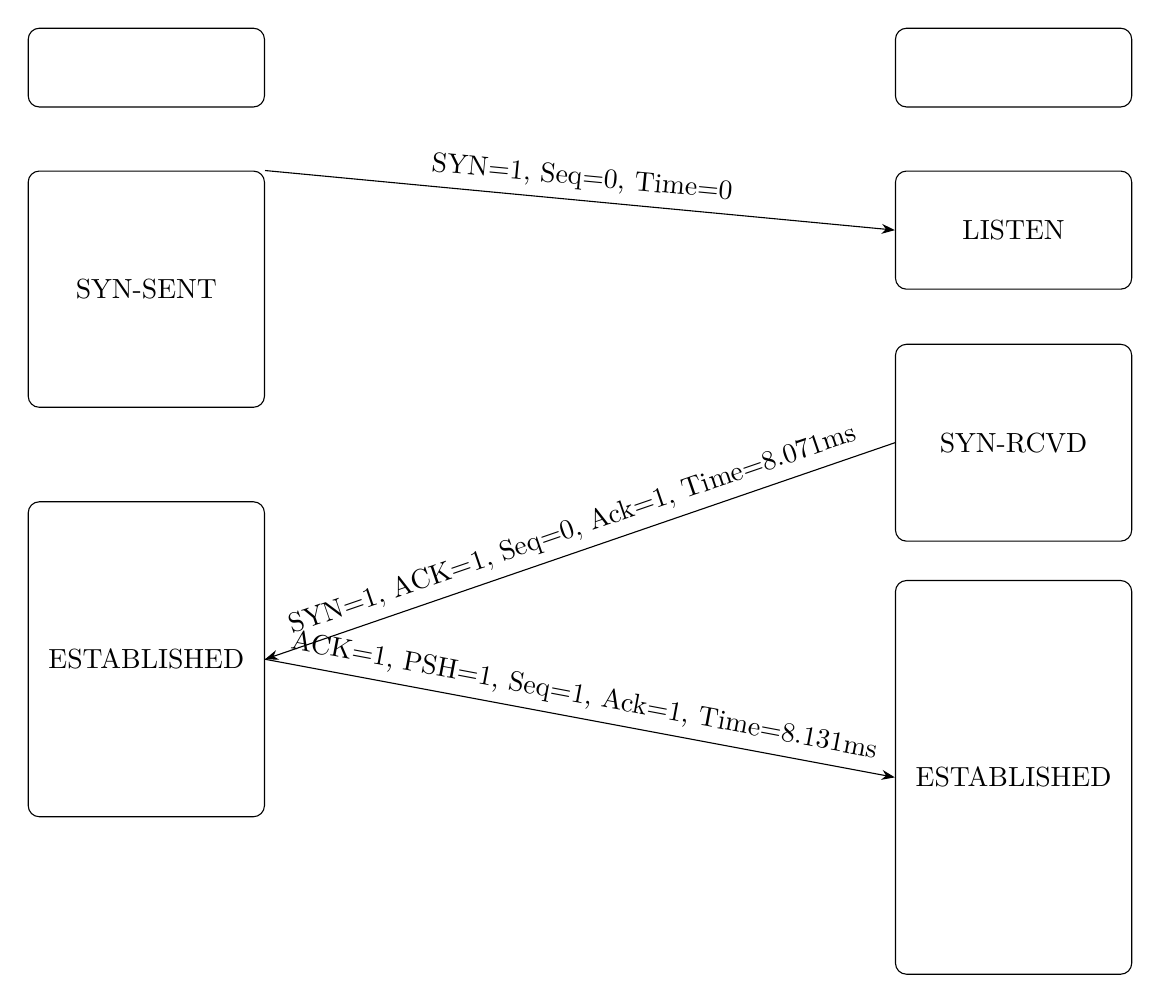
\begin{tikzpicture}[>=Stealth, node distance=2cm]
	
	% 客户机和服务器的节点
	\node[draw, rectangle, rounded corners, minimum height=1cm, minimum width=3cm] (client) {客户机};
	\node[draw, rectangle, rounded corners, minimum height=1cm, minimum width=3cm, right=8cm of client] (server) {服务器};
	
	% 状态节点
	\node[draw, rectangle, rounded corners, below=0.8cm of client, minimum height=3cm, minimum width=3cm] (syn_sent) {SYN-SENT};
	\node[draw, rectangle, rounded corners, below=0.8cm of server, minimum height=1.5cm, minimum width=3cm] (listen) {LISTEN};
	
	\node[draw, rectangle, rounded corners, below=5cm of client, minimum height=4cm, minimum width=3cm] (established_client) {ESTABLISHED};
	\node[draw, rectangle, rounded corners, below=3cm of server, minimum height=2.5cm, minimum width=3cm] (syn_rcvd) {SYN-RCVD};
	
	\node[draw, rectangle, rounded corners, below=6cm of server, minimum height=5cm, minimum width=3cm] (established_server) {ESTABLISHED};
	
	% 箭头和标签(通信过程)
	% 客户端发 SYN
	\draw[->] (syn_sent.north east) -- node[above, sloped] {SYN=1, Seq=0, Time=0} (listen.west);
	
	% 服务器回应 SYN-ACK
	% \draw[->] (listen.west) -- node[above, sloped] {SYN=1, ACK=1, seq=0, ack=1, Time=5.240} (syn_rcvd.east);
	
	% 客户端发 ACK
	\draw[->] (syn_rcvd.west) -- node[above, sloped] {SYN=1, ACK=1, Seq=0, Ack=1, Time=8.071ms} (established_client.east);
	
	% 最终确认阶段
	\draw[->] (established_client.east) -- node[above, sloped] {ACK=1, PSH=1, Seq=1, Ack=1, Time=8.131ms} (established_server.west);
	
	\end{tikzpicture}
	}
\end{center}

\begin{rmr}
	1. What TCP Options are carried on the SYN packets for your trace?
\end{rmr}

\begin{figure}[H]
	\centering
	\includegraphics[width=0.6\textwidth]{lab6/options.png}
	\caption{TCP SYN Options}
\end{figure}

\begin{ans}{Options}{Options}
根据 Wireshark 抓包获得的 Options 字段

它含有 Maximum segment size, No-Operation, Window scale, SACK permitted.

\begin{itemize}
	\item Maximum segment size: 指定最大段的大小
	\item No-Operation: 无功能(可以用于字节填充)
	\item Windows scale: 指定了窗口乘以的倍数,用于解决窗口大小的限制
	\item SACK permitted: 允许 SACK 选择性确认(乱序传输)
\end{itemize}

查阅资料得知,还有一些 SYN 包中会包含 End of Option List, Timestamp (记录时间信息) 等字段。

在这个包中,Wireshark 将 Timestamps 放置于 Options 之外,且用中括号标记,点开查看 first frame 和 previous frame 都为 0.

\end{ans}

\subsubsection{TCP Four-Way Handshake}

TCP 协议的连接释放过程,由四次握手完成,即客户端发送 FIN 包,服务器发送 ACK 包,服务器发送 FIN+ACK 包,客户端再发送 ACK 包。

\begin{figure}[H]
	\centering
	\includegraphics[width=0.8\textwidth]{lab6/FIN.png}
	\caption{TCP Four-Way Handshake}
\end{figure}

主动关闭方(180.101.50.188)发送 FIN,请求关闭连接,同时带上 ACK 确认之前的数据包。这种行为在\textbf{第一次挥手}时很常见。

根据 Wireshark 抓包获得的 Seq、Ack 字段,我们可以绘制出 TCP 四次挥手的流程图:

注意,此处的 [Time] 均为时间戳。

\begin{center}
    \resizebox{0.5\textwidth}{!}{
    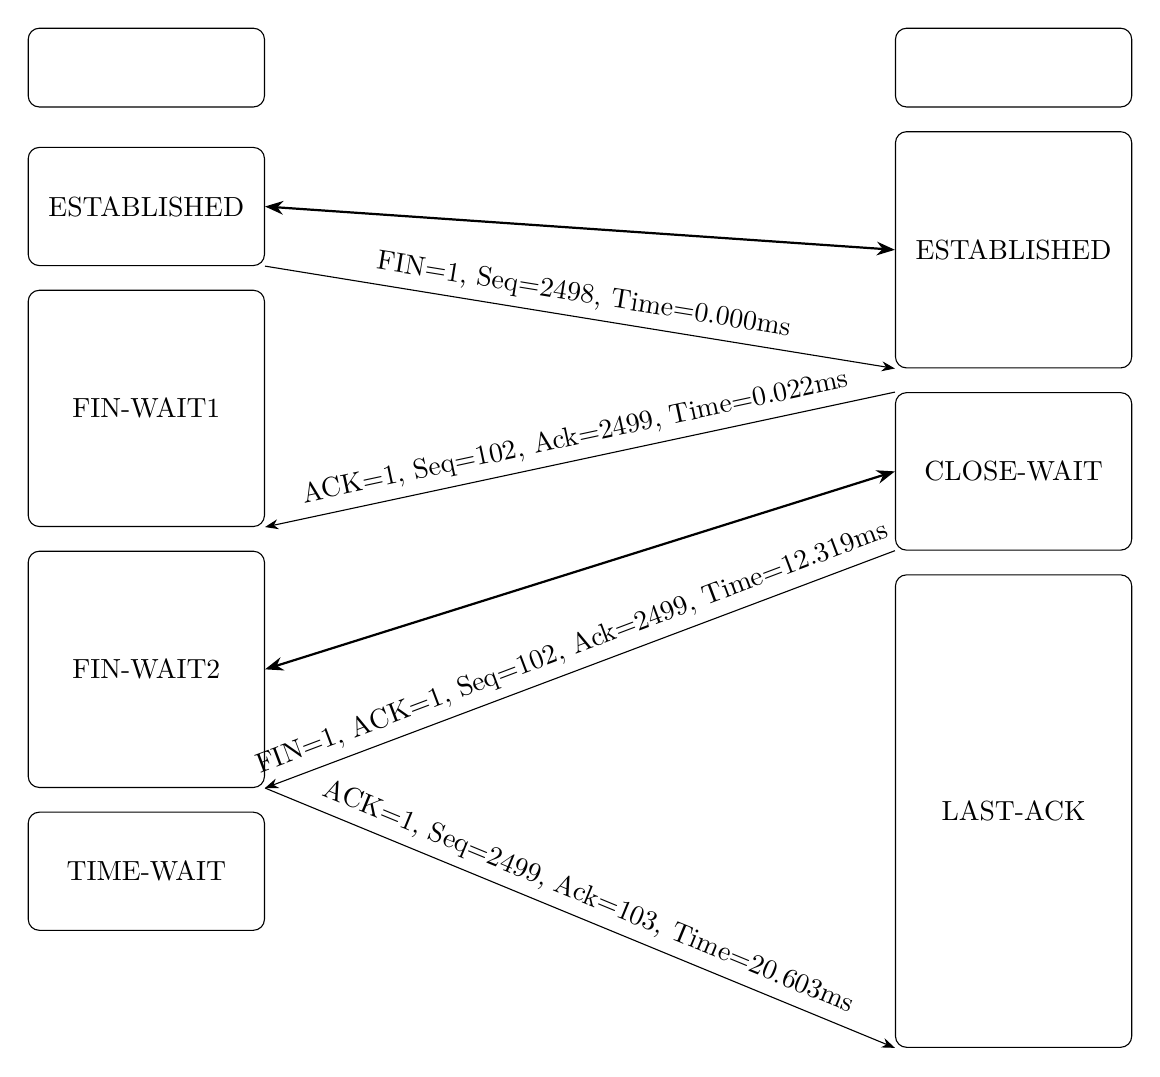
\begin{tikzpicture}[>=Stealth, node distance=2cm]
    
    % 客户机和服务器的头部节点
    \node[draw, rectangle, rounded corners, minimum height=1cm, minimum width=3cm, align=center] (client) {客户机};
    \node[draw, rectangle, rounded corners, minimum height=1cm, minimum width=3cm, right=8cm of client, align=center] (server) {服务器};

    % 客户机状态节点
    \node[draw, rectangle, rounded corners, below=0.5cm of client, minimum height=1.5cm, minimum width=3cm] (established_c) {ESTABLISHED};
    \node[draw, rectangle, rounded corners, below=0.3cm of established_c, minimum height=3cm, minimum width=3cm] (fin_wait1) {FIN-WAIT1};
    \node[draw, rectangle, rounded corners, below=0.3cm of fin_wait1, minimum height=3cm, minimum width=3cm] (fin_wait2) {FIN-WAIT2};
    \node[draw, rectangle, rounded corners, below=0.3cm of fin_wait2, minimum height=1.5cm, minimum width=3cm] (time_wait) {TIME-WAIT};
    
    % 服务器状态节点
    \node[draw, rectangle, rounded corners, below=0.3cm of server, minimum height=3cm, minimum width=3cm] (established_s) {ESTABLISHED};
    \node[draw, rectangle, rounded corners, below=0.3cm of established_s, minimum height=2cm, minimum width=3cm] (close_wait) {CLOSE-WAIT};
    \node[draw, rectangle, rounded corners, below=0.3cm of close_wait, minimum height=6cm, minimum width=3cm] (last_ack) {LAST-ACK};

    % 数据传输箭头
    \draw[<->, thick] (established_c.east) -- node[above] {数据传输} (established_s.west);

    % 第一次挥手:FIN from 客户机 to 服务器
    \draw[->] (established_c.south east) -- node[above, sloped] {FIN=1, Seq=2498, Time=0.000ms} (established_s.south west);

    % 第二次挥手:ACK from 服务器 to 客户机
    \draw[->] (close_wait.north west) -- node[above, sloped] {ACK=1, Seq=102, Ack=2499, Time=0.022ms} (fin_wait1.south east);

    % 数据传输箭头(期间)
    \draw[<->, thick] (fin_wait2.east) -- node[above, sloped] {数据传输} (close_wait.west);

    % 第三次挥手:FIN from 服务器 to 客户机
    \draw[->] (close_wait.south west) -- node[above, sloped] {FIN=1, ACK=1, Seq=102, Ack=2499, Time=12.319ms} (fin_wait2.south east);

    % 第四次挥手:ACK from 客户机 to 服务器
    \draw[->] (fin_wait2.south east) -- node[above, sloped] {ACK=1, Seq=2499, Ack=103, Time=20.603ms} (last_ack.south west);

    \end{tikzpicture}
    }
\end{center}

\begin{rmr}
	总结:为什么建立连接时使用三次握手,而释放连接时四次挥手?

	\vspace{0.5cm}

	TCP 是全双工通信,双方的关闭是独立的。

	\vspace{0.5cm}

	在建立连接时,如果是两次握手,可能会导致 “已失效的连接请求报文段” 的问题。例如,客户端发出第一个 SYN 后,若网络中断,客户端超时重试,但服务器后续接收到这个过时的 SYN,并建立错误的连接,可能造成资源浪费或通信失败。

	\vspace{0.5cm}

	而在释放连接时,客户端和服务器都需要各自发送 FIN 和确认 ACK,因此需要四次报文。
	当客户端发送 FIN 时,仅表示 “客户端完成了数据发送”,而服务器可能还在发送数据,因此服务器不能立即发送 FIN,必须等数据发送完成后才能关闭连接。
	如果是三次挥手,可能导致服务器未发送完数据就关闭连接,丢失重要数据。
\end{rmr}


\subsection{Step 5: TCP Data Transfer}

\subsubsection{获取统计信息}

在 "Static" 统计菜单下,选择 "IO 图表",以查看数据包的传输速率。

按照实验手册的说明,将间隔改为 100ms,将 Y 轴的坐标改为 Bits,

\begin{itemize}
	\item 调整过滤器为“tcp.srcport==80”仅查看下载数据包,重新绘图;
	\item 调整过滤器为“tcp.dstport==80”仅查看上传数据包,重新绘图;	
\end{itemize}

此时获得的图像如下图所示:

\begin{figure}[H]
	\centering
	\includegraphics[width=0.55\textwidth]{lab6/result.png}
	\caption{TCP Data Transfer}
\end{figure}

\subsubsection{调整图像显示}

此时图像较为不平稳,故我找了另一个大概在 100 MB 左右的文件,用于测试:

\begin{figure}[H]
	\centering
	\includegraphics[width=0.8\textwidth]{lab6/get100.png}
	\caption{Get 100 MB File}
\end{figure}

得到的结果较为可观了,接下来我们开始分析。

\begin{figure}[H]
	\centering
	\includegraphics[width=0.65\textwidth]{lab6/result2.png}
	\caption{TCP Data Transfer}
\end{figure}

\subsubsection{回答问题}

\begin{rmr}
	1.What is the rough data rate in the download direction in packets/second and bits/second once the TCP connection is running well?
	实验中的下载速率是多少? Bits/s \& packets/s
\end{rmr}

使用快捷键 X、Shift + Y 增长 X 轴,缩短 Y 轴,可以得到调整后的图像。

\begin{figure}[H]
	\centering
	\includegraphics[width=0.55\textwidth]{lab6/adjust.png}
	\caption{TCP Rough data rate}
\end{figure}

此时可以轻松看出,其速率的平均值大致在 $1.5 \times 10^7 bits/0.1s = 1.5 \times 10^8 bits/s$,最大值达到了 $2.4 \times 10^8 bits/s$。

\begin{rmr}
	What is the rough data rate in the upload direction in packets/second and bits/second due to the ACK packets?  
	实验中的上传速率,即ACK消息的发送速率是多少?
\end{rmr}

重新调整图表,将 Downloaded 方向取消显示。

\begin{figure}[H]
	\centering
	\includegraphics[width=0.55\textwidth]{lab6/adjust2.png}
	\caption{ACK Rough data rate}
\end{figure}

观察可得,平均值约为 $2.0 \times 10^6 bits/s$, 最大值达到了 $3.8 \times 10^6 bits/s$。

\begin{rmr}
	What percentage of this download rate is content? Show your calculation. To find out, look at a typical download packet; there should be many similar, large download packets. You can see how long it is, and how many bytes of TCP payload it contains.
\end{rmr}

选中一个数据包观察:

\begin{figure}[H]
	\centering
	\includegraphics[width=0.45\textwidth]{lab6/percent.png}
	\caption{TCP Packet}
\end{figure}

可以看到其总大小为 1494 字节,其中 TCP 负载部分为 1440 字节,占比约为 96.38\%.

\begin{rmr}
	If the most recently received TCP segment from the server has a sequence number of X, then what ACK number does the next transmitted TCP segment carry?
	如果最近从服务器收到的TCP数据段的序列号是X,那么下一个发送的ACK是多少?
\end{rmr}

Ack号告诉下一个期望的序列号,因此它将是X加上这一帧的TCP载荷的大小。

\subsection{Explore on your own}

\subsubsection{TCP 拥塞与 AIMD 策略}

TCP 拥塞控制使用了 AIMD(加性增大、乘性减小)策略:

\begin{itemize}
	\item 加性增大:每个 RTT 成功确认后,拥塞窗口(Congestion Window,CWND)按线性增加。
	\item 乘性减小:检测到丢包或网络拥塞时,CWND 会立即减半。
\end{itemize}

拥塞控制的四个阶段:

\begin{itemize}
	\item 慢启动(Slow Start)
	\item 拥塞避免(Congestion Avoidance)
	\item 快速重传(Fast Retransmit)
	\item 快速恢复(Fast Recovery)
\end{itemize}

\subsubsection{TCP 的可靠性机制}

TCP 通过以下机制实现可靠性:

\begin{itemize}
	\item 序列号(Sequence Number)和确认号(Acknowledgment Number)。
	\item 超时重传(Timeout Retransmission)。
	\item 快速重传(Fast Retransmit)。
	\item 滑动窗口协议。
	\item RTT 估算(Round Trip Time):动态调整超时时间。
\end{itemize}

\section{实验结果总结}

\subsection{TCP 报文结构的理解}

在实验中,我通过 Wireshark 对捕获的 TCP 数据包进行了详细分析,明确了 TCP 报文中的各个字段及其功能。

\begin{itemize}
	\item 了解了 TCP 报文头部各字段的长度和作用,例如源端口、目的端口、序列号(Sequence Number)、确认号(Acknowledgment Number)、标志位(Flags)等。
	\item 掌握了 TCP 报文中选项字段的具体内容,包括 MSS、窗口缩放因子(Window Scale)、选择性确认(SACK)等,并理解了它们对数据传输效率的影响。
\end{itemize}

\subsection{TCP 三次握手与四次挥手}

通过实验详细分析了 TCP 的连接建立(Three-Way Handshake)和释放(Four-Way Handshake)过程,明确了:

三次握手的具体步骤和目的,了解了 SYN、SYN+ACK 和 ACK 数据包的字段变化。
四次挥手中,客户端和服务器独立关闭连接的过程,解释了为什么需要四次挥手而不是三次。

\subsection{TCP 数据传输过程}

在实验中,利用 Wireshark 捕获和分析了 TCP 数据传输的过程,并从以下几个方面得到了结果:

\begin{itemize}
	\item 计算了 TCP 数据包的传输速率,包括下载方向的速率(bits/s 和 packets/s)以及 ACK 报文的上传速率。
	\item 分析了 TCP 数据包的负载比例,得出数据包的有效负载占比达 96.38\%,进一步理解了 TCP 报文的资源利用效率。
\end{itemize}

\section{附录}

\subsection*{参考资料}

\begin{itemize}
    \item 常用测速文件:\href{https://b.lxd.cc/post-323.html}{\underline{https://b.lxd.cc/post-323.html}}
\end{itemize}

\end{document}